\section{Корпус изделия}
В соответствии с техническим заданием был разработан корпус для тонкого клиента.
Трехмерная модель корпуса представлена на рисунке (см. рисунок~\ref{pic:case}), сборка
изделия — на рисунке (см. рисунок~\ref{pic:assy}).

Фотографии изделия в сборе представлены на
рисунках~\ref{pic:assy_photo_1},~\ref{pic:assy_photo_2}.

\begin{figure}[h]
    \center
    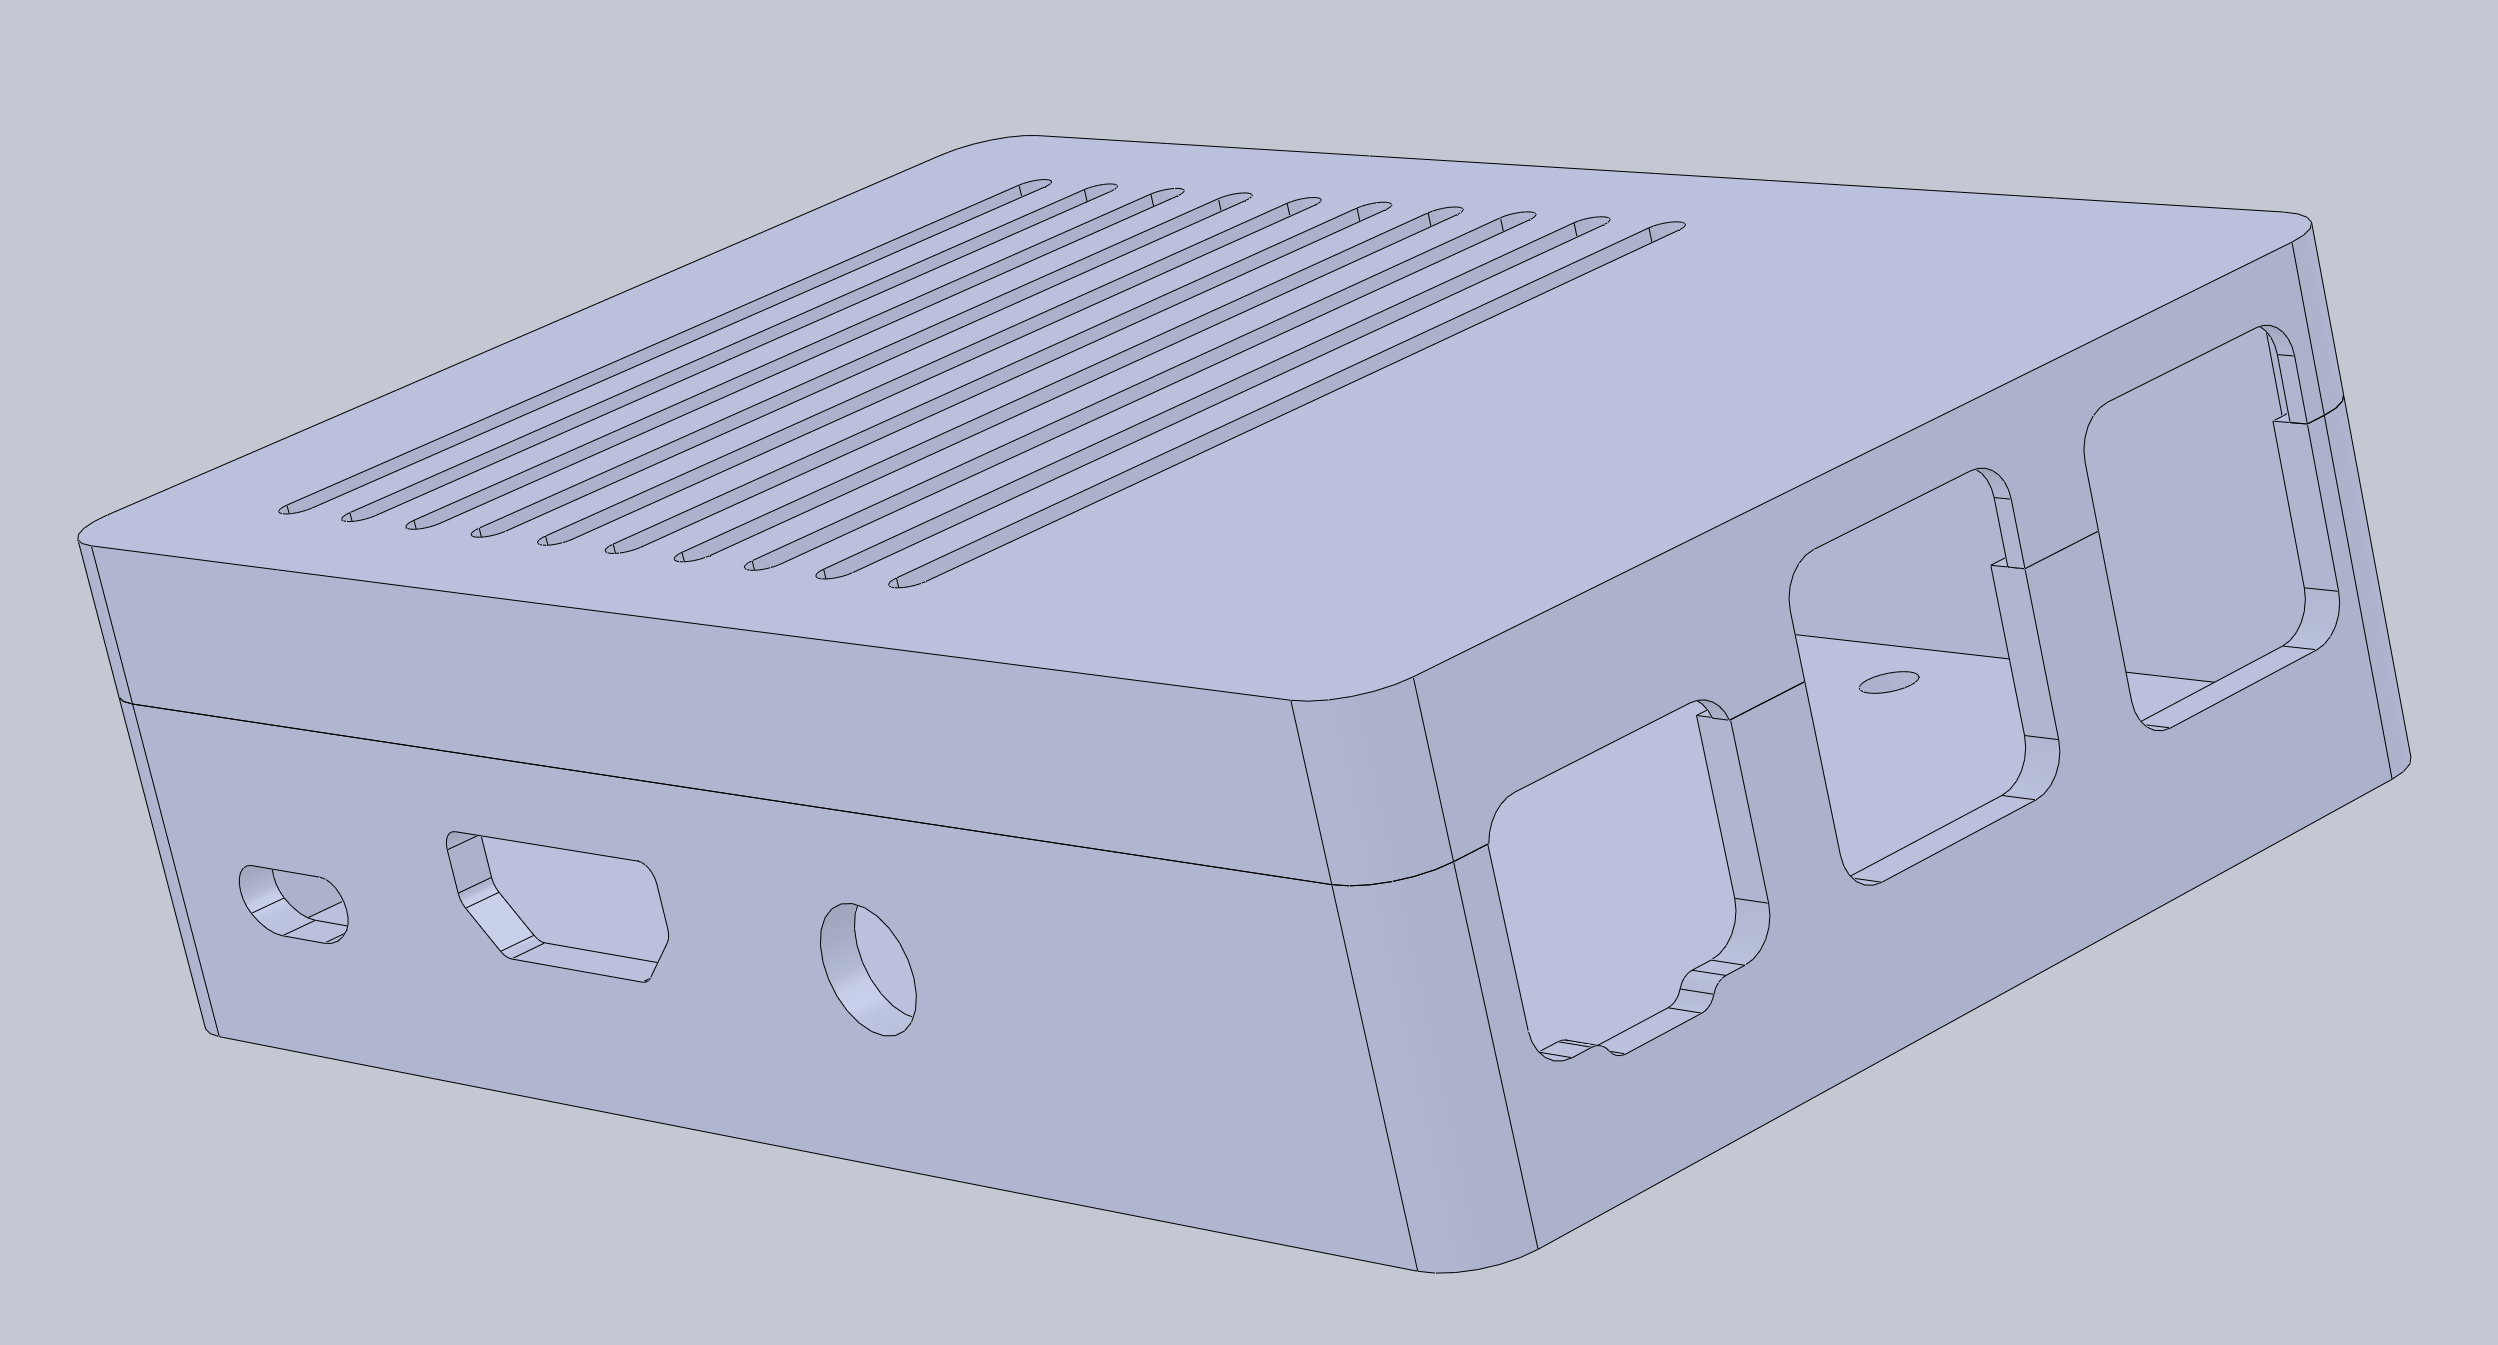
\includegraphics[height=6cm]{case}
    \caption{Модель корпуса}
    \label{pic:case}
\end{figure}

\begin{figure}[h]
    \center
    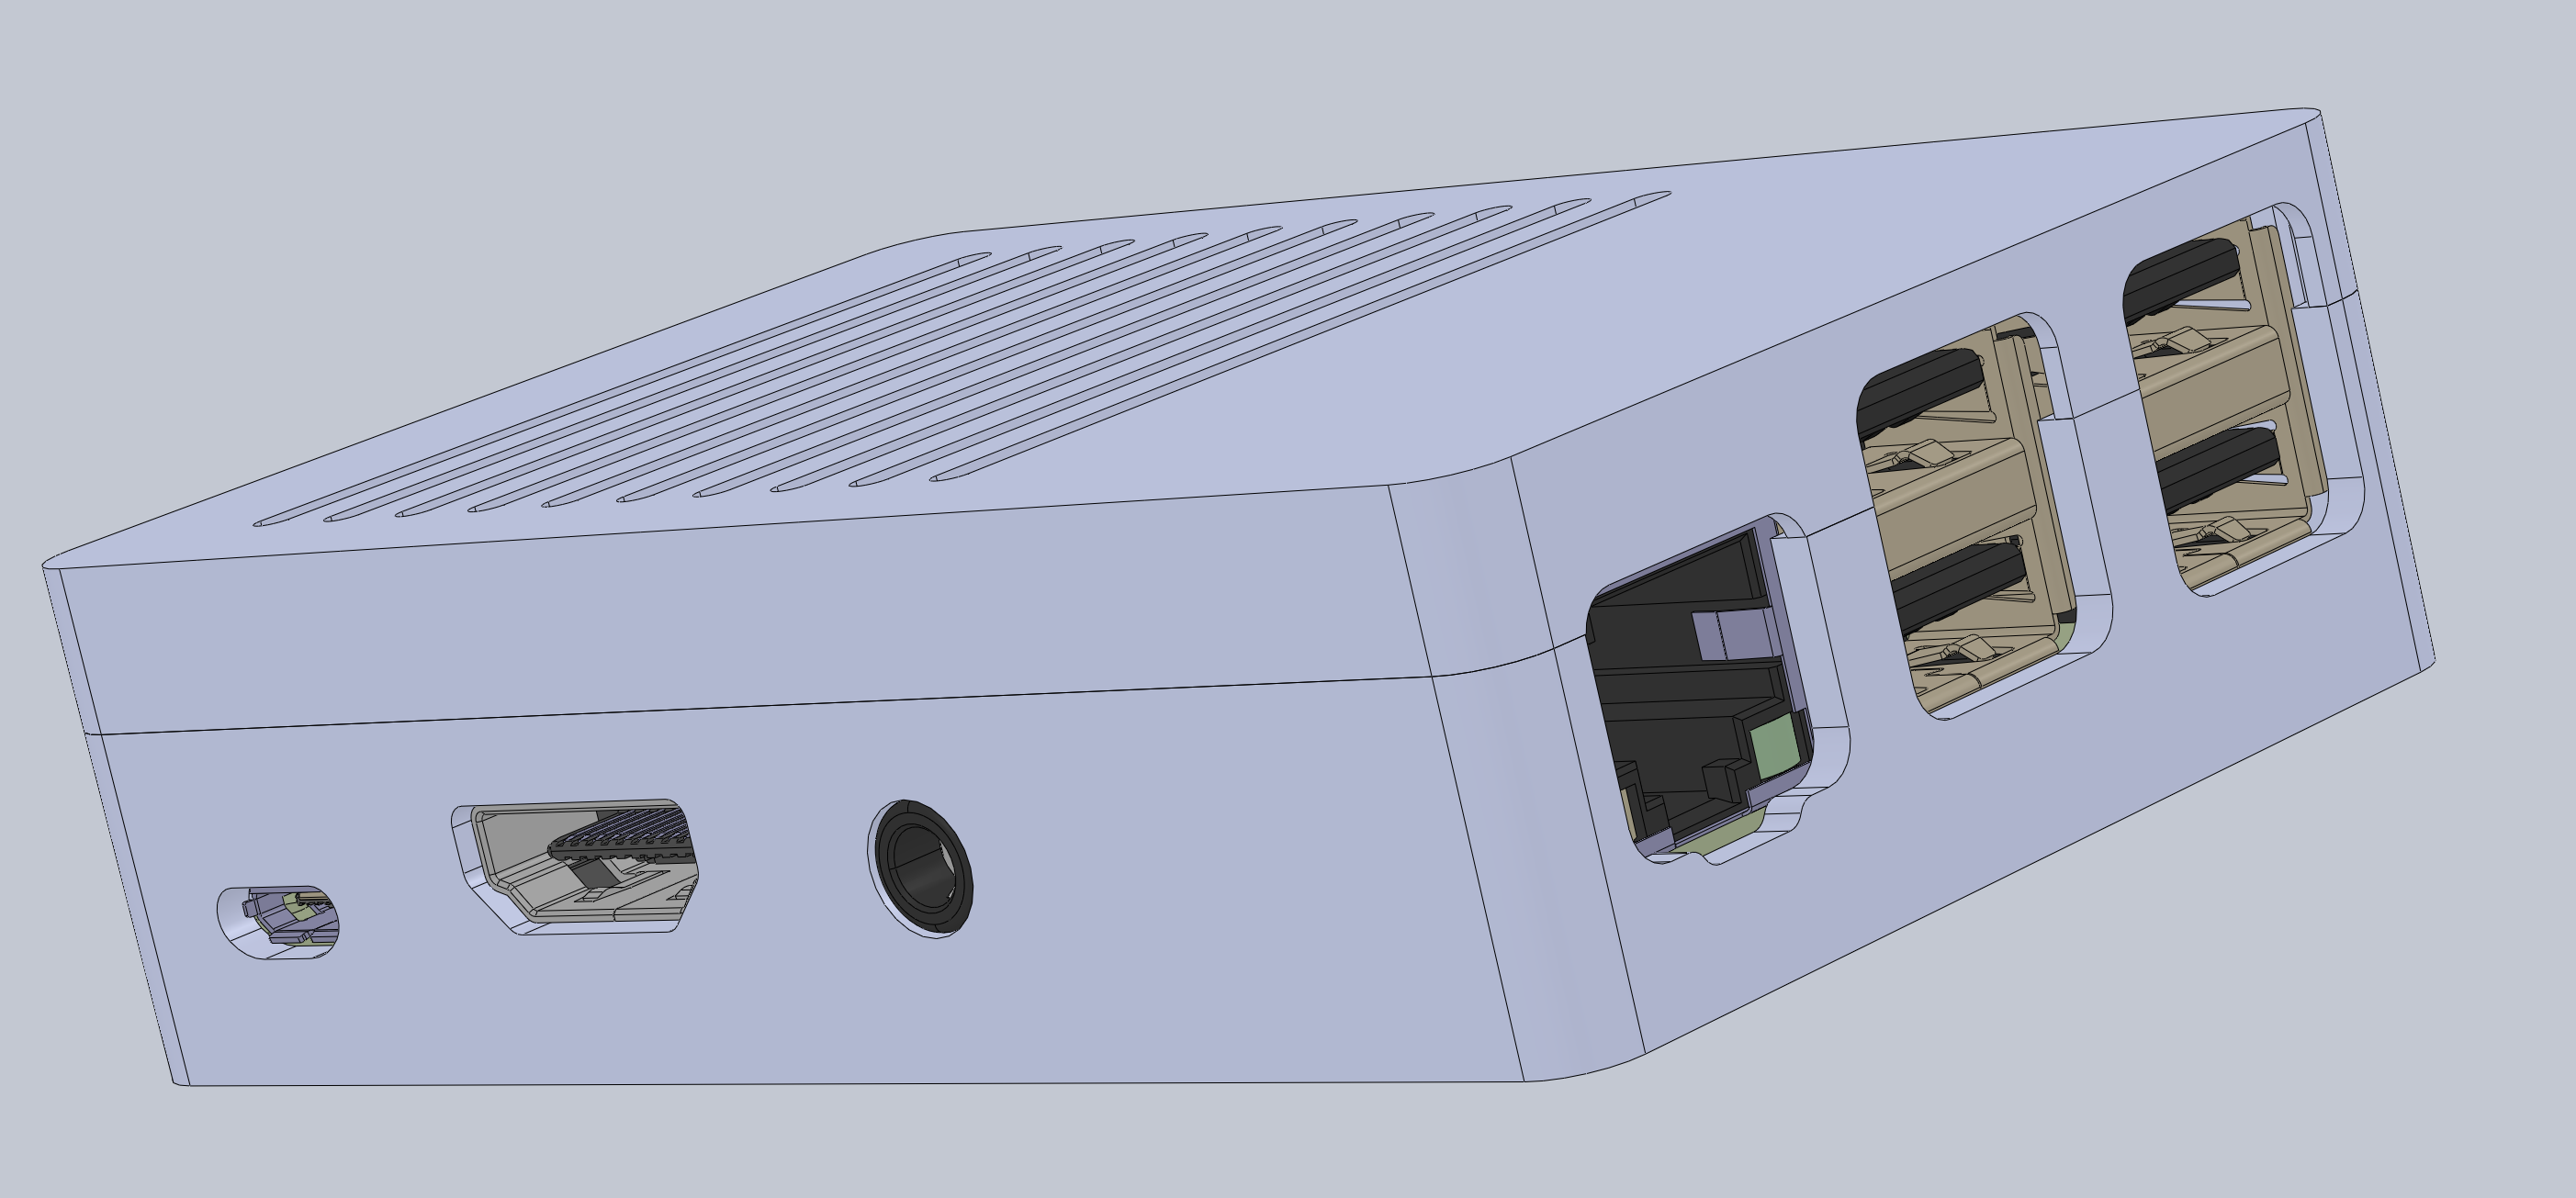
\includegraphics[height=8cm]{assy}
    \caption{Модель сборки}
    \label{pic:assy}
\end{figure}

\begin{figure}[h]
    \center
    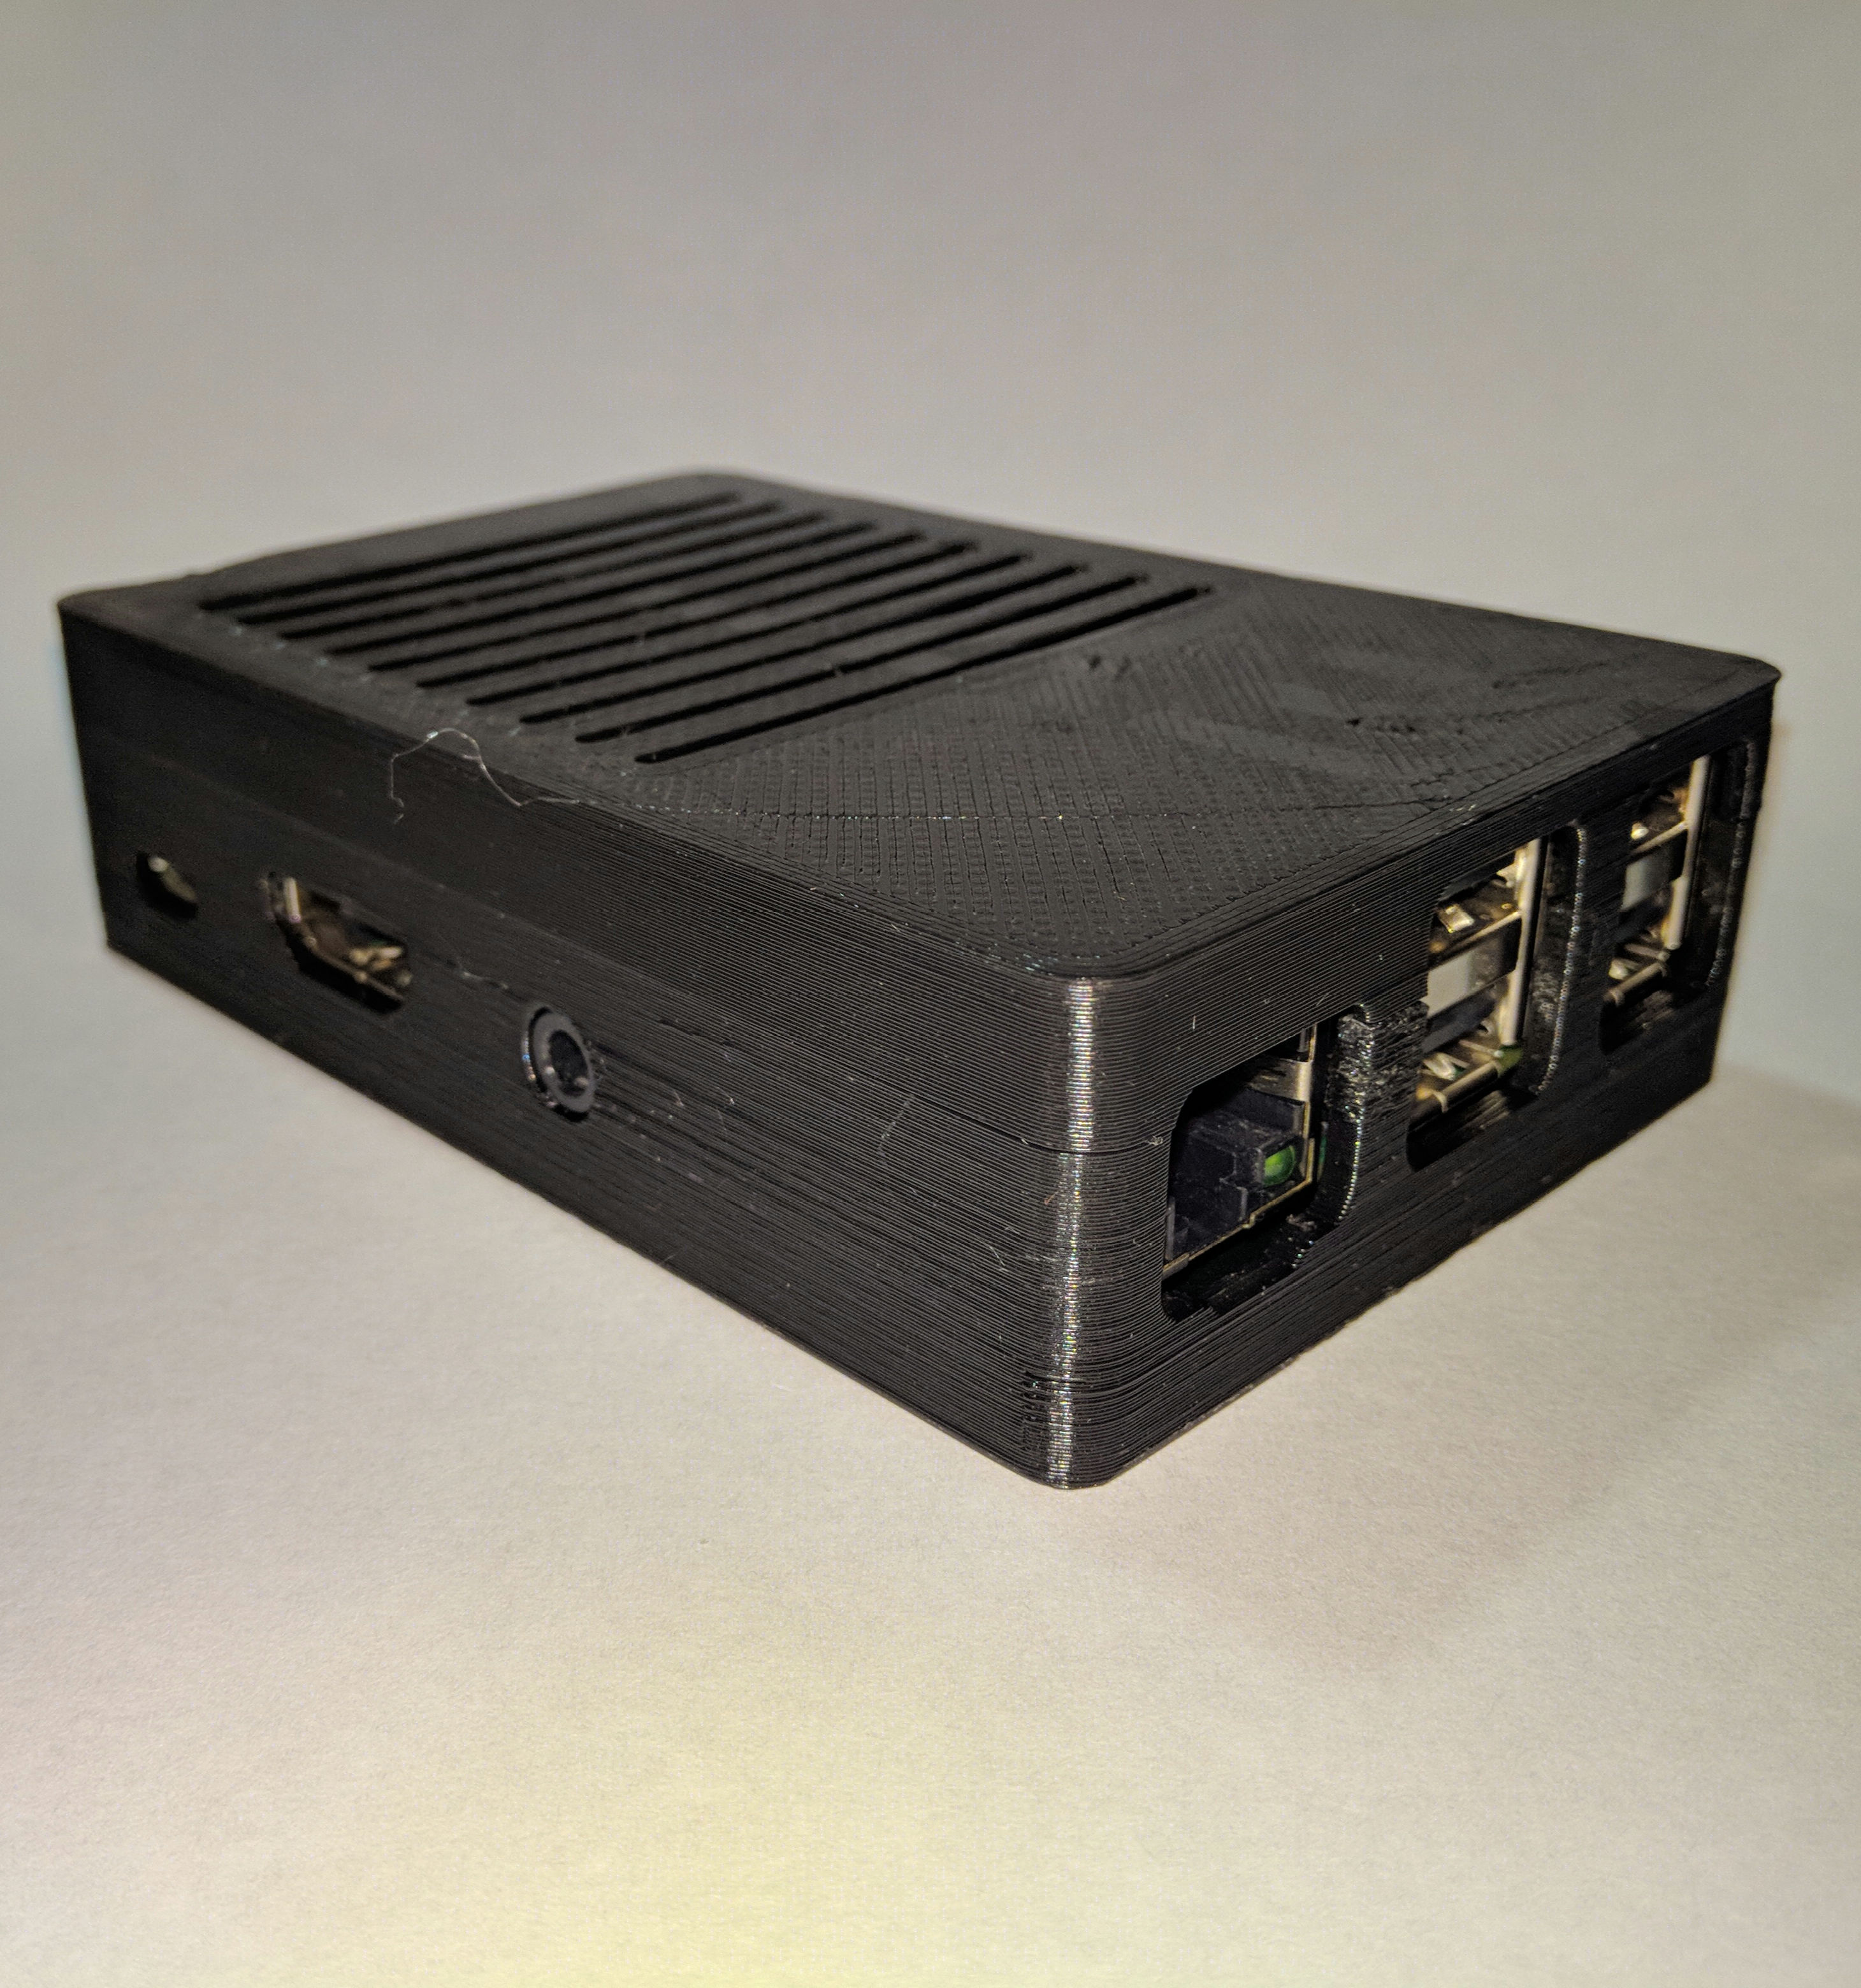
\includegraphics[height=10cm]{assy_photo_1}
    \caption{Устройство в сборе}
    \label{pic:assy_photo_1}
\end{figure}

\begin{figure}[h]
    \center
    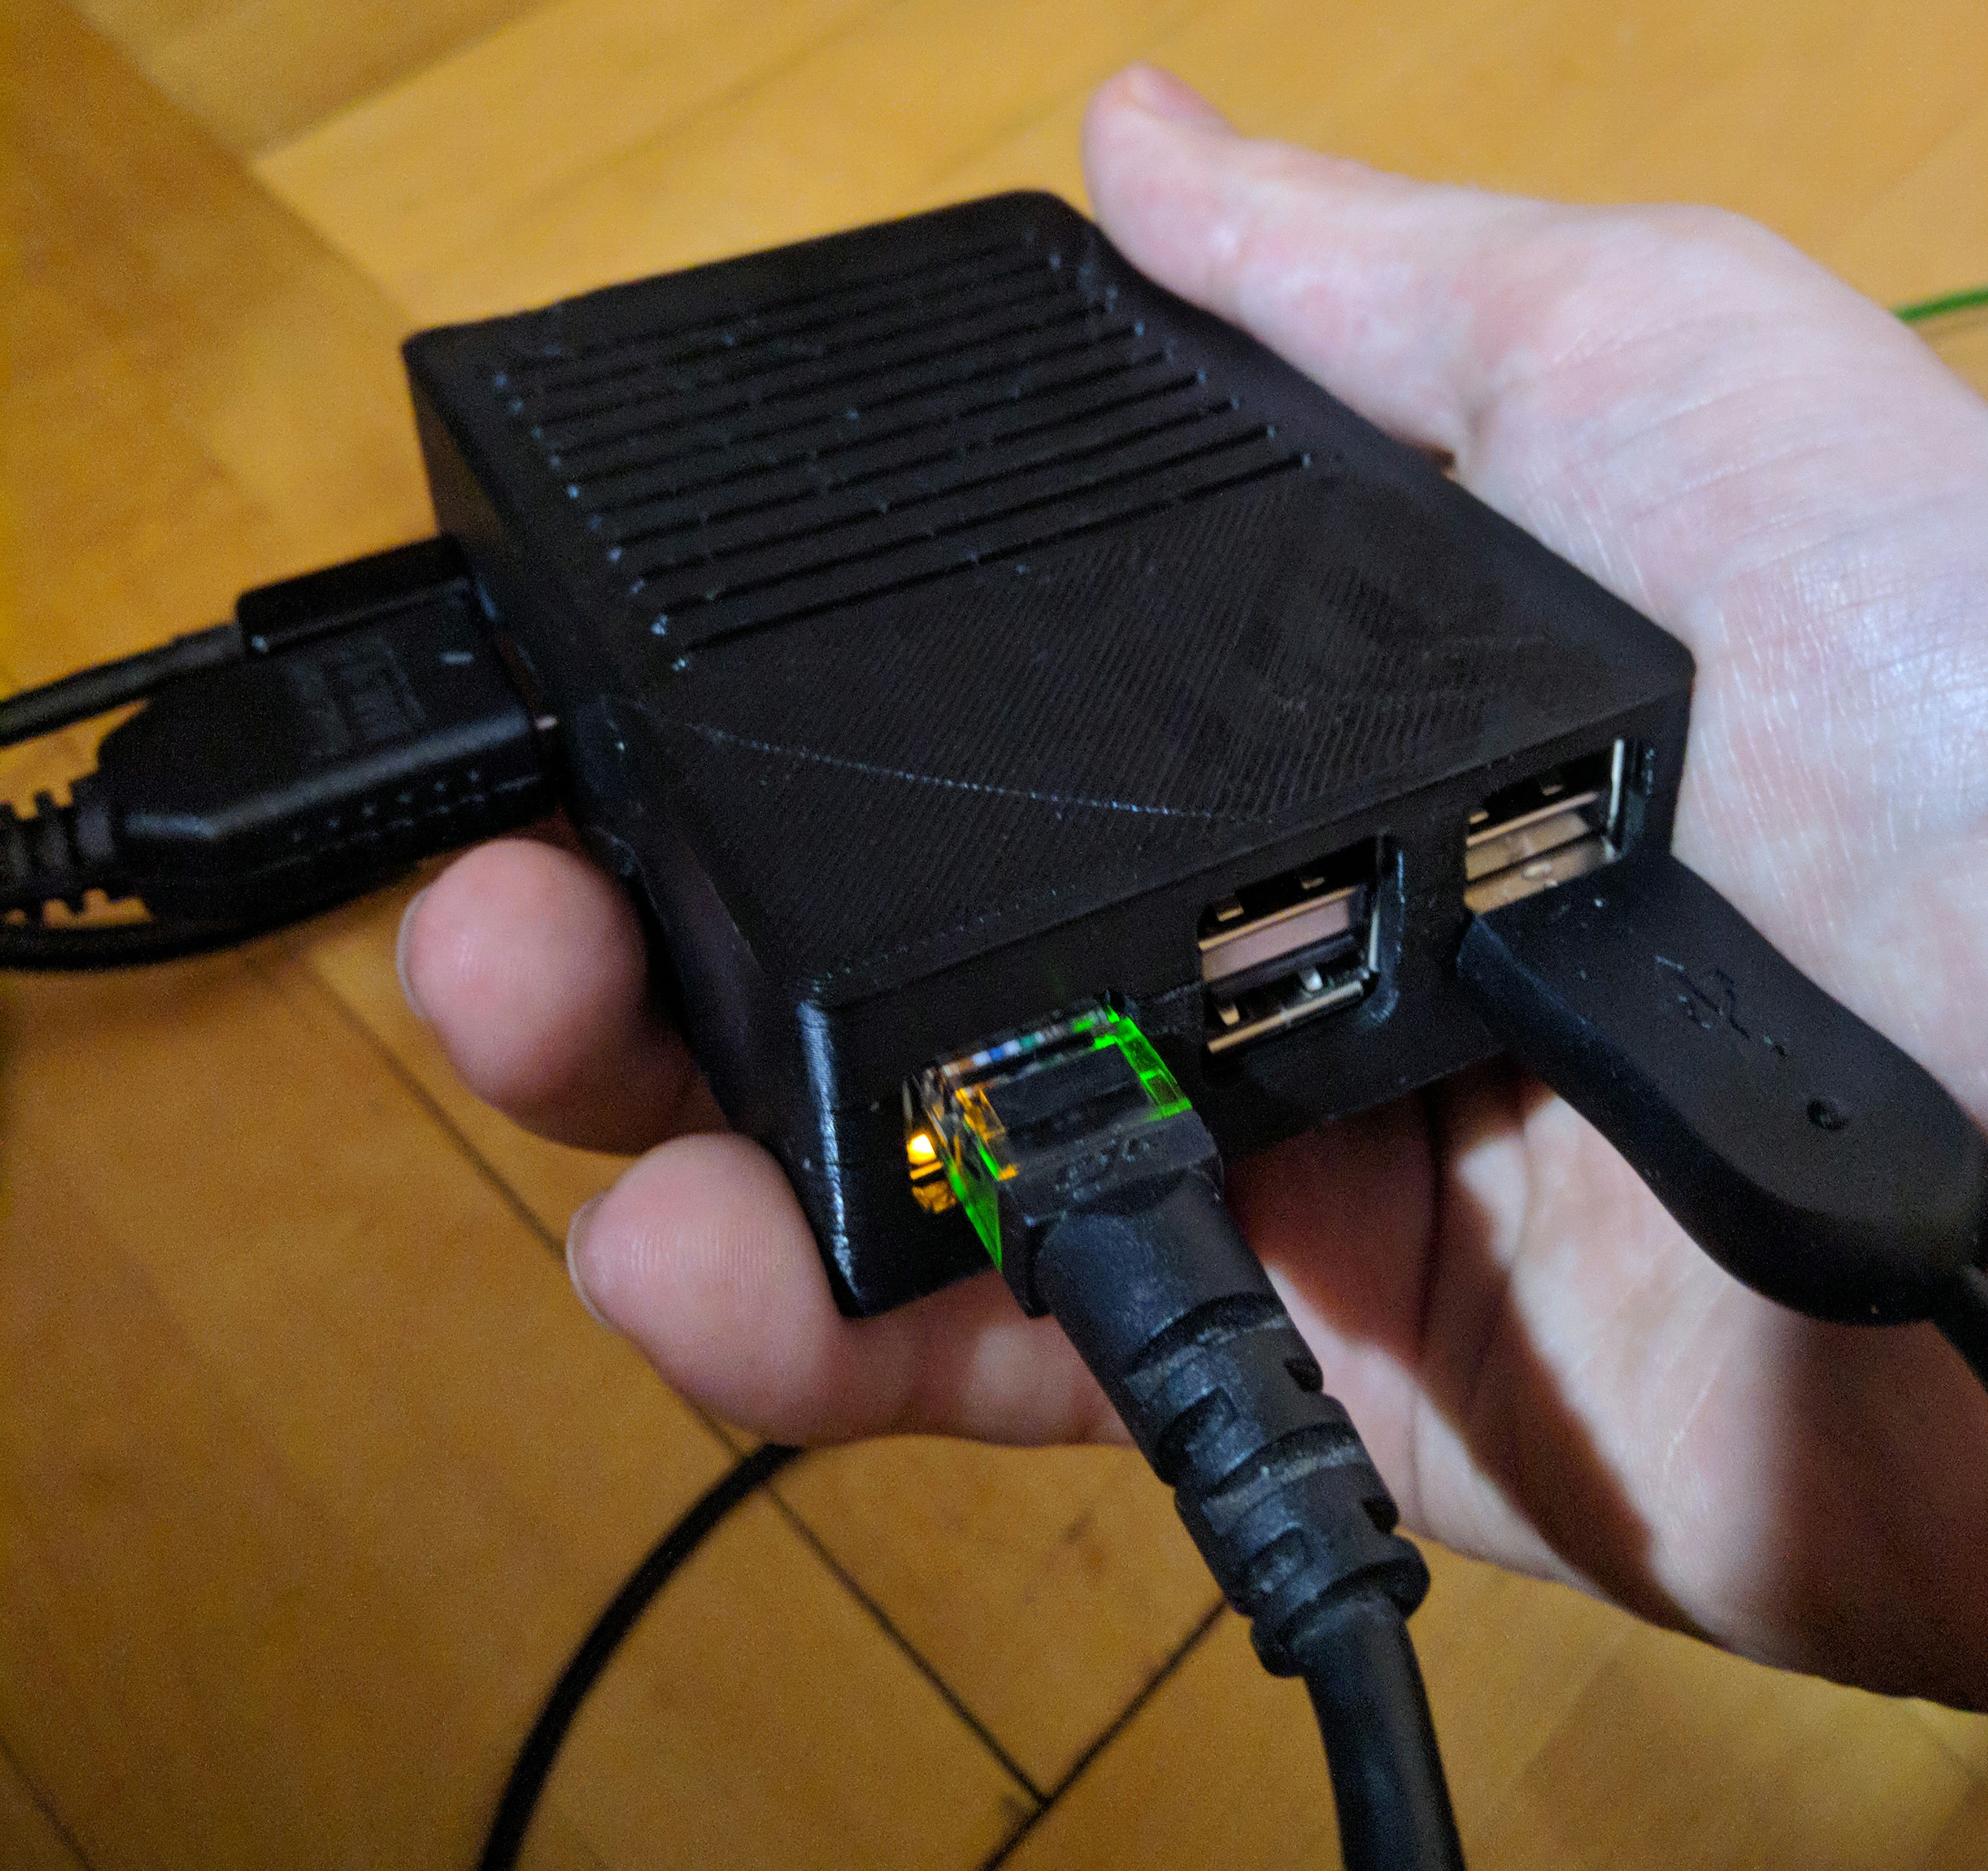
\includegraphics[width=\linewidth]{assy_photo_2}
    \caption{Устройство в работе}
    \label{pic:assy_photo_2}
\end{figure}
